\pdfoutput=1
\documentclass[twocolumn]{aastex62}
%%\documentclass[]{emulateapj}

%Accepted/received/... %%

\received{xxx}
\revised{yyy}
\accepted{zzz}

%% Command to document which AAS Journal the manuscript was submitted to.
\submitjournal{AAS Journals}

%% Short title/authors

\shorttitle{LXUV History of TRAPPIST-1}
\shortauthors{Fleming et al.}

%% Begin document, title, packages %%
\usepackage{hyperref}
\usepackage{xspace}
\usepackage{graphicx}
\usepackage{amsmath}
\usepackage[caption=false]{subfig}

%% Custom commands
\def\mearth{{\rm\,M_\oplus}}
\def\rearth{{\rm\,R_\oplus}}
\def\msun{{\rm\,M_\odot}}
\def\rsun{{\rm\,R_\odot}}
\def\lsun{{\rm\,L_\odot}}
\def\gsim{~\rlap{$>$}{\lower 1.0ex\hbox{$\sim$}}}
\def\lsim{~\rlap{$<$}{\lower 1.0ex\hbox{$\sim$}}}

\newcommand{\xxx}[1]{{\textbf{#1}}}
\newcommand{\vplanet}[0]{\texttt{VPLanet}\xspace}
\newcommand{\approxposterior}[0]{\texttt{approxposterior}\xspace}
\newcommand{\eqtide}[0]{\texttt{EQTIDE}\xspace}
\newcommand{\stellar}[0]{\texttt{STELLAR}\xspace}
\newcommand{\kepler}[0]{\textit{Kepler}\xspace}

%% Begin doc %%
\begin{document}

\title{On The XUV Luminosity Evolution of TRAPPIST-1}

%% AUTHORS %%

%%\correspondingauthor{David P. Fleming}
%%\email{dflemin3@uw.edu}

%%\author[0000-0001-9293-4043]{David P. Fleming}
\author{David P. Fleming}
\affil{Astronomy Department, University of Washington \\
Box 951580, Seattle, WA 98195}
\affil{NASA Astrobiology Institute - Virtual Planetary Laboratory Lead Team, USA}

\author{Rory Barnes}
\affiliation{Astronomy Department, University of Washington \\
Box 951580, Seattle, WA 98195}
\affil{NASA Astrobiology Institute - Virtual Planetary Laboratory Lead Team, USA}

\author{Rodrigo Luger}
\affil{NASA Astrobiology Institute - Virtual Planetary Laboratory Lead Team, USA}
\affiliation{Center for Computational Astrophysics, Flatiron Institute \\
New York, NY 10010}

%% ABSTRACT %%

\begin{abstract}

Abstract.

- we constrain the stellar evolution and mass of TRAPPIST-1 using best priors and constraints currently available. we make our posterior distributions available for use with water loss simulations as the FXUV is a core input to such models, be it energy limited or recombination limited, maybe non-thermal escape models as well (look into that). our model and machine learning approach is all open source and documented on github, including a repo for the project itself
- TRAPPIST-1 conference stellar evolution stuff is 1st day, so email invited talks presenters and send them draft and thank them for their work which I use and cite in my own work - adam burgasser and jeff linsky
- 5 plots/tables: table of priors; corner plot; L, LXUV, R sampled from posteriors; \approxposterior comparison plot with distributions on top of each other 
- \citet{vanGrootel2018} decided luminosity and age were best constraints as R and Teff are unreliable for stellar models.  see their paper for a good discussion on this point and for good references to cite how metallicity or magnetic fields or incorrect opacity sources can lead to this discrepancy. See Filippazzo 2015 and Luger 2017 for additional age constraints to cite. Also from Burgasser 2017, "must be young based on the strength of its nonthermal magnetic emission (Bourrier et al. 2017; O’Malley-James Kaltenegger 2017"
- cite scholnik papers saying UV/Xray measurements of M dwarfs are critical, especially to estimate water losses and cite other HAZMAT papers for the activity evolution of M dwarfs
- note why I chose LXUV evolution as a function of time and not Rossby number, e.g. why I didn't use Wright+2018 data explicitely
- from Peacock+2018: "Late-type M stars remain UV active for much longer than their early M counterparts, typically with more variability in the FUV than the NUV (Miles Shkolnik 2017)."
- Roettenbacher+2017 show that the Prot measurement might not be reliable, mention Brett's TRAPPIST-1 work for how the rotation period might not be 3 d

\end{abstract}

%% Keywords %%

\keywords{}

%% Intro %%

\section{Introduction} \label{sec:intro}

Introduction.

%% Methods %%

\section{Methods} \label{sec:methods}

\subsection{Markov Chain Monte Carlo} \label{sec:methods:mcmc}

MCMC!

\subsection{Priors} \label{sec:methods:priors}

Priors!

-\citet{Jackson2012} $f_{sat}$ measurements are derived for late K dwarfs through early F dwarfs, but are consistent with observations of fully-convective M dwarfs \citep{Wright2018}
- Jackson 2019 for M dwarf radius inflation
- great info on characterization from \citet{Burgasser2017}: "As spin-down timescales increase for
the lowest-mass stars, saturated magnetic emission can persist
for even slowly rotating stars (P less than 86 day) with little
correlation between the incidence of emission and rotation
period (West et al. 2008, 2015)"

\begin{deluxetable}{lcc}
\tabletypesize{\small}
\tablecaption{Prior Distributions \label{tab:priors}}
\tablewidth{0pt}
\tablehead{
\colhead{Parameter} & \colhead{Prior} & \colhead{Notes}
}
\startdata
$m_\star$ [$M_{\odot}$] & $\mathcal{U}(0.07, 0.11)$ & Uniform \\  
$f_{sat}$ & $\mathcal{N}(-3.14, 0.37^2)$ & \citet{Jackson2012} \\
$t_{sat}$ [Gyr] & $\mathcal{U}(0.1, 12)$ & Uniform \\
$t_{age}$ [Gyr] & $\mathcal{N}(7.6, 2.2^2)$ & \citet{Burgasser2017} \\
$\beta_{XUV}$ & $\mathcal{N}(-1.18, 0.31^2)$ & \citet{Jackson2012}
\enddata \vspace*{0.1in}
\end{deluxetable}

%% Results %%

\section{Results} \label{sec:results}

Results.

\begin{figure*}[ht]
	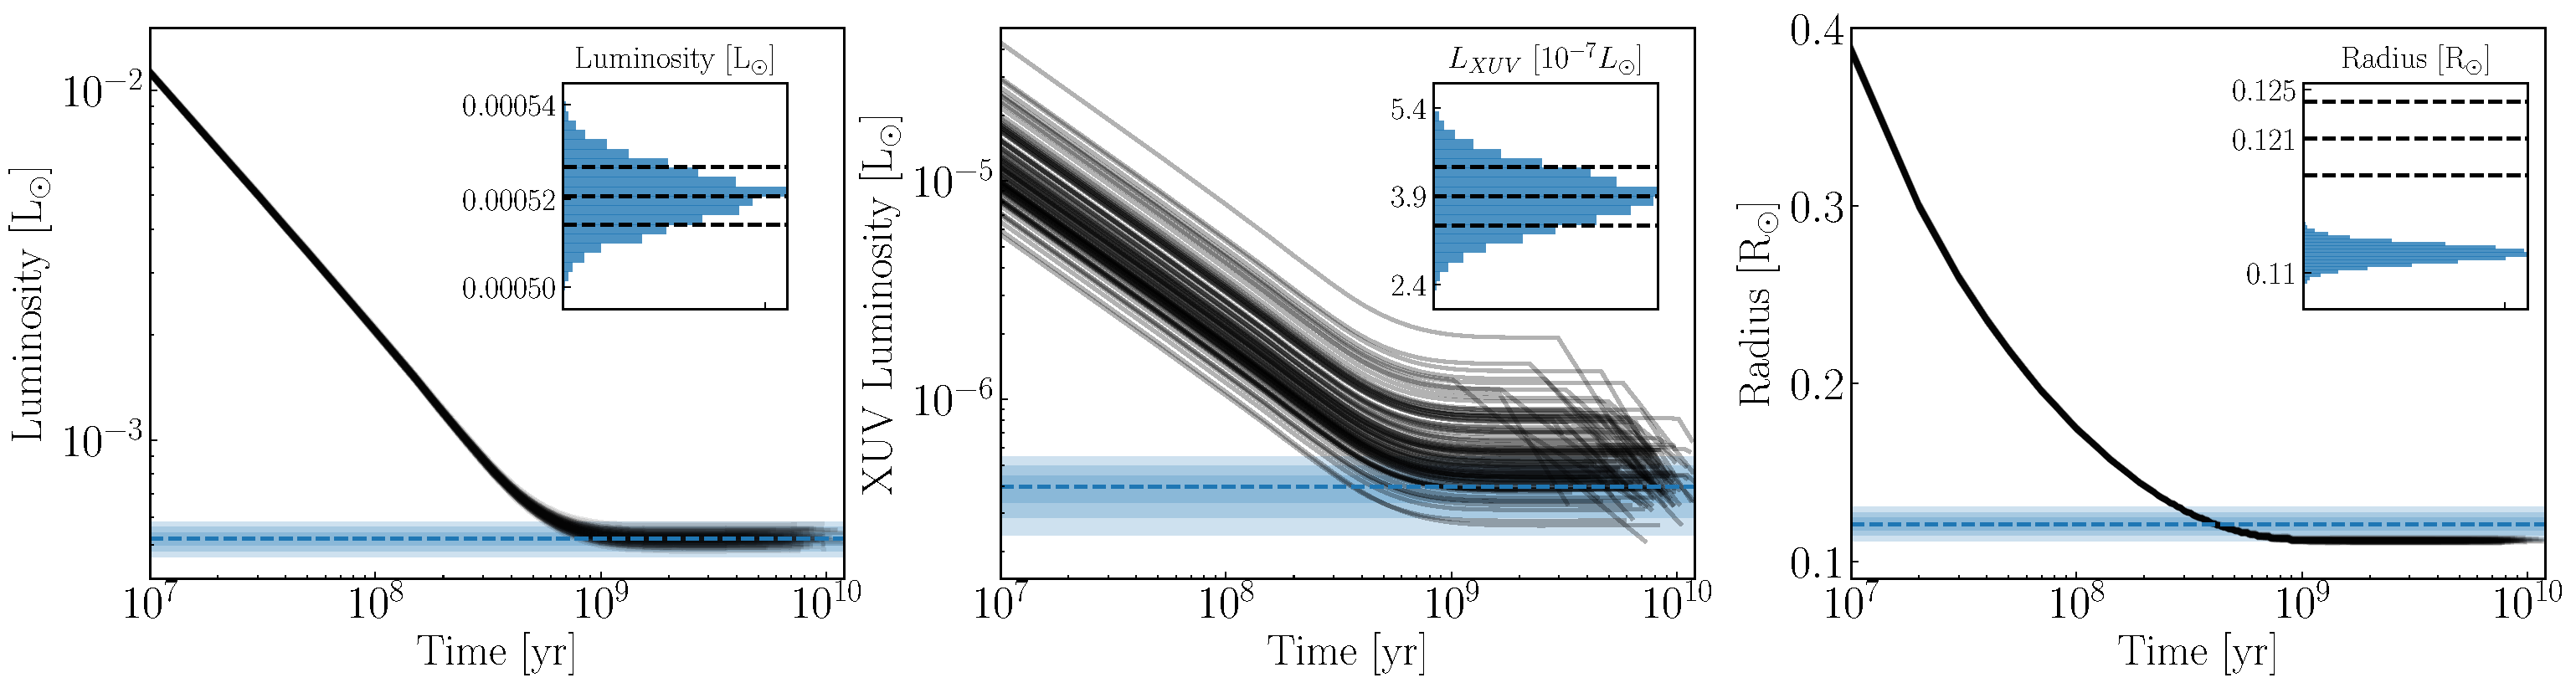
\includegraphics[width=\textwidth]{../Analysis/Evol/trappist1Evol.pdf}
   \caption{Caption.}%
    \label{fig:evol}%
\end{figure*}

%% approxposterior %%

\section{\approxposterior} \label{sec:approx}

Results.

%% Discussion %%

\section{Discussion} \label{sec:discussion}

Discuss!

%% ACKNOWLEDGEMENTS %%
\acknowledgments
This work was facilitated though the use of advanced computational, storage, and networking infrastructure provided by the Hyak supercomputer system and funded by the Student Technology Fund at the University of Washington. DPF was supported by NASA Headquarters under the NASA Earth and Space Science Fellowship Program - Grant 80NSSC17K0482.  RB acknowledges support from the NASA Astrobiology Institute's Virtual Planetary Laboratory under Cooperative Agreement number NNA13AA93A.

%% SOFTWARE %%
\software{matplotlib: \citet{Hunter2007}, numpy: \citet{vanderWalt2011}, \vplanet: \citet{Barnes2016,vplanet2018}}, \approxposterior: \citet{FlemingVanderPlas2018}

%% BIBLIOGRAPHY %%

\bibliography{trappist}

% End of file
\end{document}